\documentclass[conference]{IEEEtran}
\IEEEoverridecommandlockouts
% The preceding line is only needed to identify funding in the first footnote. If that is unneeded, please comment it out.
\usepackage{cite}
\usepackage[utf8]{inputenc}
\usepackage[brazil]{babel}
\usepackage[T1]{fontenc}
\usepackage{amsmath,amssymb,amsfonts}
\usepackage{algorithmic}
\usepackage{graphicx}
\usepackage{textcomp}
\def\BibTeX{{\rm B\kern-.05em{\sc i\kern-.025em b}\kern-.08em
    T\kern-.1667em\lower.7ex\hbox{E}\kern-.125emX}}
\begin{document}

\title{Unidade Remota de Irrigação\\}

\author{\IEEEauthorblockN{Ivan Carlos da Silva Lopes}
\IEEEauthorblockA{\textit{Departamento de Engenharia Elétrica} \\
\textit{Universidade Federal Fluminense}\\
Niterói, Brasil \\\
ivanlopes$@$id.uff.br}
}

\maketitle

\begin{abstract}

O presente trabalho apresenta o projeto de uma unidade remota de irrigação destinada a pequena propriedades. São apresentadas as lógicas de operação que constituem o software da unidade desenvolvida, bem como o hardware básico a ser utilizado, sem a especificação de modelos. É realizada uma simulação e um teste com protótipo para aferir o funcionamento dos subsistemas da unidade remota.

\end{abstract}

\begin{IEEEkeywords}
Sistema Embarcado, Irrigação Autônoma, ATmega328P, Sistema Autônomo, Acionamento Remoto
\end{IEEEkeywords}

\section{Introdução}

O presente projeto se caracteriza pelo desenvolvimento de um sistema de irrigação remoto, de fácil utilização, confiável e de baixo custo, a fim de possibilitar a irrigação de pequenas propriedades. Com tal sistema, espera-se facilitar o cultivo de hortas e pomares em propriedades de agricultura familiar, que constituem aproximadamente 84\% [1] das propriedades rurais brasileiras. Espera-se também contribuir para a promoção do cultivo de plantas como hobbie o que, segundo [2], promove inclusive a manutenção da biodiversidade e preservação de pequenas espécies de insetos e plantas nativas, além do bem-estar pessoal de quem cultiva tal hábito saudável.


O objetivo deste trabalho é desenvolver algumas tecnologias para a automação de uma horta/plantação, se baseando principalmente em diminuir os custos para o acesso dessa tecnologia a um público mais amplo. Sendo assim, esse trabalho irá focar principalmente no uso do microcontrolador ESP8266 para esse fim, devido ao seu baixo custo. Toda a comunicação de controle será feita via WiFi, que é o meio de comunicação do ESP8266. Toda a parte eletrônica foi projetada para poder ser colocada em uma Placa PCB, de forma a ficar pronta para instalação em seus devidos ambientes e que permita atualizações e a resolução de problemas de software via USB. Logo, neste trabalho foi desenvolvido uma tecnologia, um sistema para acionar até 12 bombas ou válvulas via WiFi, com o ESP8266 acionando o relé que ligaria a válvula solenoide respectiva à saída desejada, quando esse relé conectado a um interruptor de forma a fazer uma ligação \textit{threeway}, que permite que tanto o relé quanto o interruptor acionem a válvula. Todo o controle e acionamento dos dispositivos deve ser feito via celular, ou outros dispositivos com comunicação WiFi, que estejam conectados à rede local.

\section{Projeto Básico}

O projeto básico da unidade de irrigação deve contemplar os requisitos estabelecidos pelo escopo do projeto, a saber, um sistema de irrigação que funcione de forma ininterrupta, com independência do usuário e relativo grau de autonomia, ou seja, capaz de tomar decisões. Como a irrigação será realizada com base em um horário determinado pelo usuário, o primeiro requisito a ser atendido é a contagem do tempo na URI, na escala humana de segundos, minutos e horas. Tal mecanismo de contagem é comumente chamado na literatura e em sistemas embarcados e de automação de \textit{Real-Time Clock} (relógio de tempo real), ou \textit{RTC} \cite{b1}. A unidade contará também com um sistema de comunicação sem fio, para realização de comando e monitoramento por parte do usuário.

Outro requisito do sistema diz respeito à água utilizada para a irrigação, a ser armazenada em um reservatório próprio para a unidade. O nível do reservatório deve ser monitorado a fim de que a devida operação da irrigação não seja impedida por falta de água. Deseja-se ainda que o reservatório seja, se possível, realimentado de forma autônoma, ou que o usuário seja alertado quanto ao nível crítico das condições necessárias para irrigação. Devem ser monitoradas também as condições climáticas e do solo, para que a irrigação seja condizente com as necessidades locais, sem fornecer água em excesso ou falta. Dessa forma, a operação de irrigação será condicionada às condições locais de forma a atuar de forma mais eficiente e em concordância com as necessidades da vegetação.

Relativo aos equipamentos e dispositivos utilizados, o projeto básico contempla o uso de um microcontrolador ATmega328P,  onde será executado a programação, uma placa ESP8266 para a realização da comunicação sem fio, sensores de nível e umidade do solo, um reservatório, para o acumulo da água a ser utilizada e válvulas para realização do controle do fluxo de água. O sistema deve contar ainda com uma fonte alternada de $127 V$, para alimentação das válvulas, e uma fonte contínua de $5 V$, para alimentação dos circuitos eletrônicos. Na Fig. \ref{fig1}, pode-se perceber o esquema ilustrativo simplificado da unidade de irrigação e suas conexões em nível de equipamentos e componentes.

\begin{figure}[htbp]
\centerline{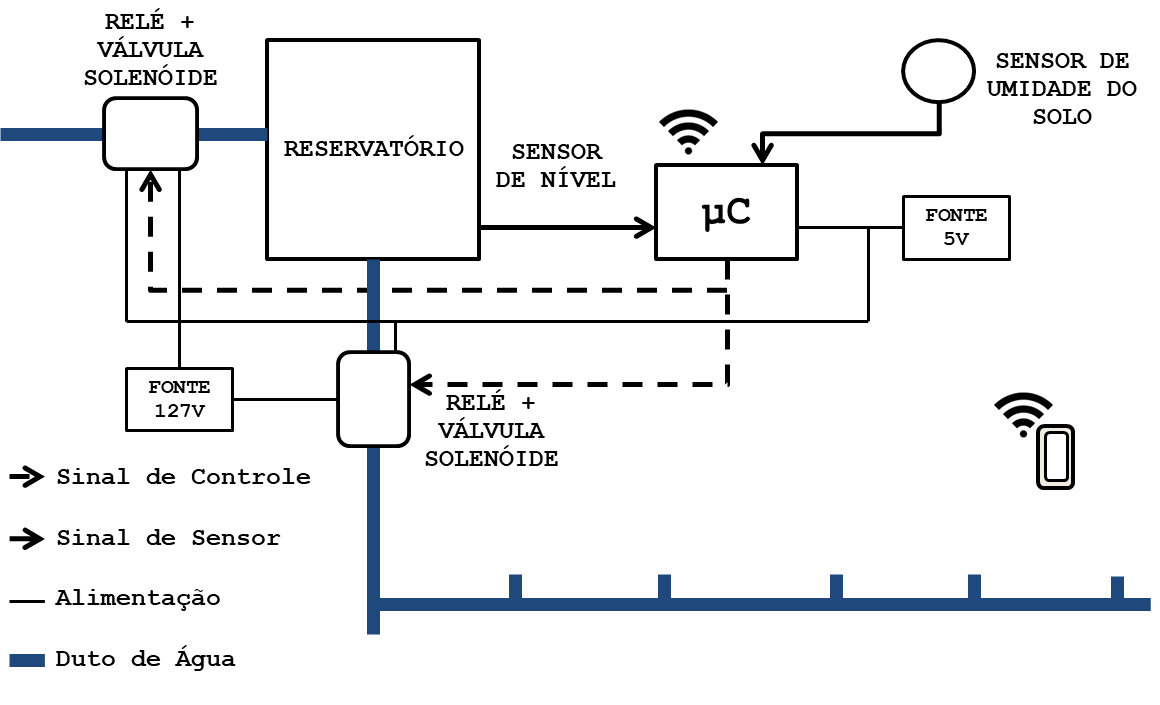
\includegraphics[angle=0, scale=.2]{Img1.png}}
\caption{Esquema simplificado do projeto básico.}
\label{fig1}
\end{figure}

Na Fig. \ref{fig2}, é explicitado fluxo de informações entre os subsistemas da unidade remota de irrigação. O referido \textit{RTC} marca a passagem de tempo, comunicando-o ao subsistema de acionamento do motor. No tempo determinado, este opera sujeito ainda às condições reportadas pelos sensores e pela comunicação sem fio com o usuário, que, por sua vez, também recebe o status das condições locais vindas dos sensores, caso solicitado pelo usuário. A comunicação sem fio é utilizada ainda para atualização do relógio, impedindo que este perca a sua precisão, e para a configuração inicial das variáveis do relógio.

\begin{figure}[htbp]
\centerline{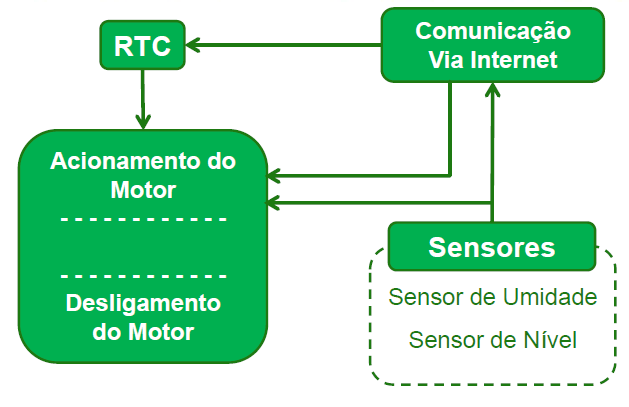
\includegraphics[angle=0, scale=.3]{Img2.png}}
\caption{Fluxo de informações entre os subsistemas.}
\label{fig2}
\end{figure}

\subsection{Real-Time Clock}

Em sistemas embarcados e de automação, é comum o uso de \textit{RTC}’s, principalmente com o emprego de módulos externos, cujas características são possuir alimentação e cristal próprios. Dessa forma, a contagem de tempo torna independente do clock do microcontrolador utilizado no sistema, podendo ser realizada de forma muito mais precisa, uma vez que o módulo é dedicado para este fim e possui um clock mais adequado para o mesmo, com frequência milhares de vezes menor que o do microprocessador, geralmente. A alimentação própria, realizada por meio de uma bateria, assegura o funcionamento do \textit{RTC} mesmo quando o sistema principal encontra-se totalmente desligado, o que garante confiabilidade e robustez ao sistema e permite que, depois de inicialmente configurada a hora, esta não necessite mais ser reconfigurada.

A fim de minimizar os custos e aproveitar ao máximo o potencial do microprocessador ATmega328P, optou-se por não incluir na unidade de irrigação um módulo \textit{RTC} externo, mas sim desenvolver dentro do próprio microcontrolador um mecanismo de contagem de tempo em escala real. Este mecanismo é bem similar ao apresentado em \cite{b1} e consiste na utilização de um dos temporizadores fornecidos pelo microcontrolador e de interrupções para, de certa forma, simular o funcionamento das engrenagens de um relógio real.

A cada número $CM$ de ciclos de máquina, aciona-se uma interrupção, que incrementa uma variável $tic$, como o tic-tac em um relógio. Por sua vez, a cada certo número $ntic$ de $tic$’s conta-se um segundo. A partir da contagem de segundos, definem-se os minutos e horas através de sub-rotinas que se comunicam, constituindo o motor do relógio. Para a definição dos valores de ciclo de máquina CM e número de $tic$’s , foram realizadas as seguintes operações. Em (\ref{eq1}), definiu-se o período do contador com base no prescaler escolhido, de 256, e no clock do controlador, de 16MHz. $CM$, expressa pelo contador $OCR0A$ do \textit{Timer 0}, foi arbitrada como $250$ e o número de $tic$'s foi calculado com em (\ref{eq2}).

\begin{equation}
T = \frac{256}{16e^6} = 1.6e^{-5}
\label{eq1}
\end{equation}

$CM = OCR0A = 250;$

\begin{equation}
ntics = \frac{1seg}{T\times OCR0A} = 250
\label{eq2}
\end{equation}

Logo, a cada $250$ ciclos de máquina, ativar-se-á a interrupção, que contará um $tic$. A cada $250$ $tic$’s, contar-se-á um segundo. Com a medição dos segundos, tem-se os valores de minutos e horas. Os valores são atualizados sempre que o sistema for inicializado e, após, a cada hora, para que a precisão seja assegurada. Dessa forma, ainda é mantida relativa independência em relação à comunicação sem fio, sendo o sistema capaz de operar mesmo sem a atualização constante.

\subsection{Acionamento do Válvula}

A válvula escolhida para realizar o controle do fluxo de água foi uma válvula do tipo solenoide, acionada quando excitada por tensão alternada de $127 V$. Por isso, para o acionamento pelo microcontrolador, optou-se pela utilização de um relé de $5 V$ para comunicação dos equipamentos. Porém, ao se utilizar tais relés, existe o risco da ocorrência de picos de tensão vindos da bobina do relé, ou de não se alcançar a corrente mínima de operação do relé. Portanto, faz-se conveniente a utilização de um transistor ou optoacoplador para isolar os equipamentos e garantir a corrente necessária. Na unidade de irrigação, decidiu-se por utilizar um optoacoplador de modelo 4N25.

Para o acionamento do relé, deve ser atribuída a uma das saídas um valor lógico $1$ e, para o desligamento, um valor lógico $0$. Dessa forma, pode ser utilizado mais um conjunto válvula e relé, ou válvula e bomba, tanto para o controle do fluxo de água quanto para realimentação do reservatório, atribuindo à unidade um caráter customizável.

\subsection{Sensoriamento}

Os sensores na unidade remota de irrigação possuem a função de monitorar as condições do ambiente para promover uma operação mais eficiente e adequada, e monitorar as condições do sistema para verificar a capacidade de operação. Como já mencionado, os sensores utilizados são dois: um sensor de umidade do solo e um sensor de nível para o reservatório.

Com base no estado do solo expresso pelo sensor de umidade, é selecionado um dentre três tempos de irrigação, correspondendo às necessidades do solo. Os tempos de irrigação são $15$, $10$ e $5$ minutos, relativos à irrigação máxima, média e mínima, respectivamente. Em caso de mau funcionamento do sensor, é utilizado o tempo de irrigação médio. O projeto contempla ainda a possibilidade de leitura do valor de umidade a qualquer momento pelo usuário, de forma remota.

A cada irrigação, é verificado o nível do reservatório. Caso o sensor de nível exprima um sinal referente ao atingimento do nível crítico de água, envia-se uma mensagem para o usuário, alertando sobre a necessidade da reposição da água para irrigação, ou aciona-se uma válvula ou bomba, realimentado automaticamente o reservatório, com um tempo de operação e vazão ajustados à capacidade do reservatório.

\subsection{Comunicação Sem Fio}

A comunicação sem fio será realizada através de um módulo ESP8266. O ESP8266 é um microcontrolador produzido pela empresa Espressif Systems. Esse microcontrolador possui um sistema de comunicação WiFi próprio, que é o seu grande diferencial. Por esse motivo ele é largamente utilizado como módulo WiFi para outros microcontroladores, como o Arduíno, por exemplo, apesar de possuir um processador próprio, e de ser possível utilizar somente o ESP8266 para criar sistemas embarcados. Uma vantagem do ESP8266 é o seu baixo custo, geralmente na faixa de 20 a 50 reais. O Esp8266 está no mercado desde 2014, o que faz com que ainda existam poucos artigos e trabalhos sobre ele. A principal publicação sobre o mesmo é \cite{b2}, que demonstra quais são as formas de programar o ESP8266 e quais são as suas utilidades, bem como a eletrônica necessária para realizar os projetos demonstrados.

Existem diversos tipos de modelos do ESP8266, como o ESP-1, ESP-12, Esp Olimex por exemplo. Como o processador é o mesmo para todos os modelos do ESP8266, mudando apenas o número de pinos de entrada e saída (GPIO) disponíveis, memória disponível e o espaçamento entre os pinos, com isso, foi escolhido se utilizar o NODEMCU, por ele ter um número razoável de entradas e saídas para esse projeto e pela facilidade de obtê-lo.

\subsection{Comunicação Arduino e ESP8266}
O padrão encontrado para estabelecer a comunicação entre o ESP8266 e o Arduino foi o protocolo $I^2C$ (Inter-Integrated Circuit) que consiste em um barramento serial multimestre desenvolvido pela Philips. Sendo assim, estes usam uma estratégia master-slave, onde o microcontrolador toma o papel de master, que ao gerar o sinal de relógio comanda a troca de dados com o outro dispositivo (o slave).
No projeto, o ESP8266 tem o papel de mestre (placa controladora) e o Arduino de escravo, pois a gerência da placa com Arduino é feita pelo ESP8266.

\subsection{Comunicação Web com o ESP8266}
O ESP8266 que que no caso desempenha o papel de master no projeto, recebeu uma API REST, para comunicação, que possibilita até cinco dispositivos conectados pelo wifi ao mesmo tempo, tais como
celulares e ou paginas web.


\begin{table}[htbp]
\caption{Tabela geral de especificações do ESP8266.}
\begin{center}
\begin{tabular}{|c|c|}
\hline
Voltagem & 3.3 \\
\hline
Consumo de Corrente & 10 µA \\
\hline
Memória Flash & 16MB max (512k normal) \\
\hline
Processador & Tensilica L106 32 bit \\
\hline
Velocidade do processador & 80-160MHz \\
\hline
RAM & 32K + 80K \\
\hline
GPIOs & 17(multiplexada com outras funções) \\
\hline
Suporte 802.11 & b/g/n/d/e/i/k/r \\
\hline
\end{tabular}
\label{tab1}
\end{center}
\end{table}

\section{Simulação}

Utilizando o software de simulação de circuitos eletrônicos \textit{Proteus}, realizou-se a simulação do circuito principal de acionamento do motor, constituído pelo microcontrolador ATmega328P, pelo optoacoplador, pelo relé e por uma lâmpada alimentada por $127 V$, simbolizando o acionamento do motor. Foi configurada o horário inicial do relógio, um horário de acionamento e um horário de desligamento da lâmpada representando a válvula. Para a simulação, foi adicionada ao \textit{Proteus} uma biblioteca contendo placas de Arduino, para que se pudesse utilizar o microcontrolador ATmega328P de forma mais simplificada, como posteriormente foi feito na prática. Ao se iniciar a simulação, decorrido o tempo esperado entre o tempo inicial configurado e o tempo de acionamento, a lâmpada acendeu e, de igual forma, decorrido o tempo configurado para permanência da saída acionada, a lâmpada se apagou. Dessa forma, constatou-se a correta operação do sistema principal da unidade remota de irrigação. O digrama utilizado, explicitando o circuito, é mostrado na Fig. \ref{fig3}.

\begin{figure}[htbp]
\centerline{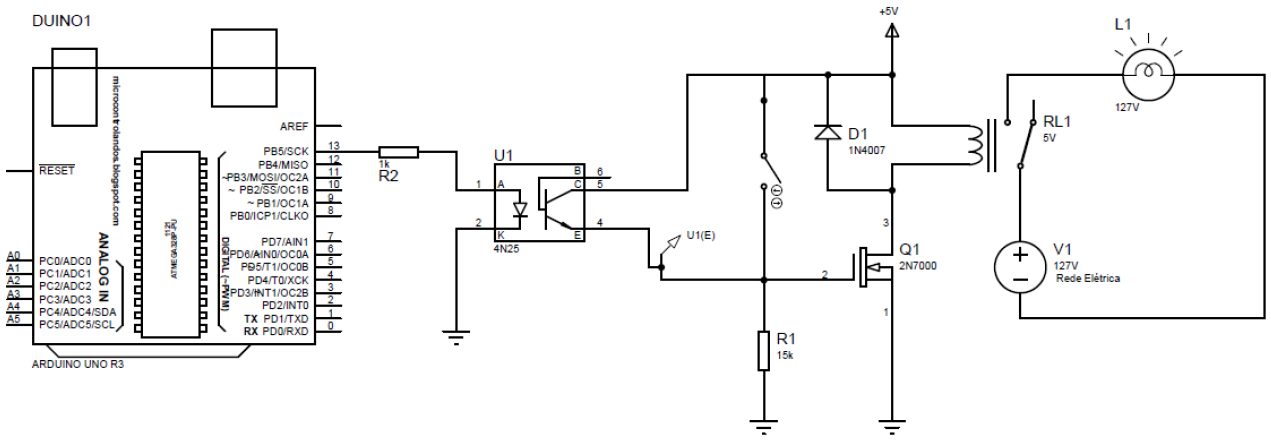
\includegraphics[angle=0, scale=.2]{Img3.png}}
\caption{Diagrama utilizado no \textit{Proteus} para a simulação.}
\label{fig3}
\end{figure}

Ademais, foi montado um protótipo para teste da comunicação entre a placa ESP8266 e o microcontrolador, também coordenando o acionamento e desligamento de um LED. A configuração da placa ESP8266 foi realizada e a conexão bem sucedida, tanto com a Internet, quanto com a placa Arduino utilizada no teste. A partir dessa conexão, podem ser alcançados os objetivos iniciais do projeto, no que diz respeito à comunicação com o usuário, tanto para recebimento de sinais de controle quanto para relatórios de status do sistema e dos sensores. Podem ser alcançados também os objetivos referentes a comunicação com o sistema principal, no que diz respeito à atualização dos valores do relógio, tanto no momento da inicialização quanto de hora em hora, para manutenção da sincronia. A Fig. \ref{fig4} apresenta um esquema simplificado da conexão da placa ESP8266 com a placa Arduino Uno.

\begin{figure}[htbp]
\centerline{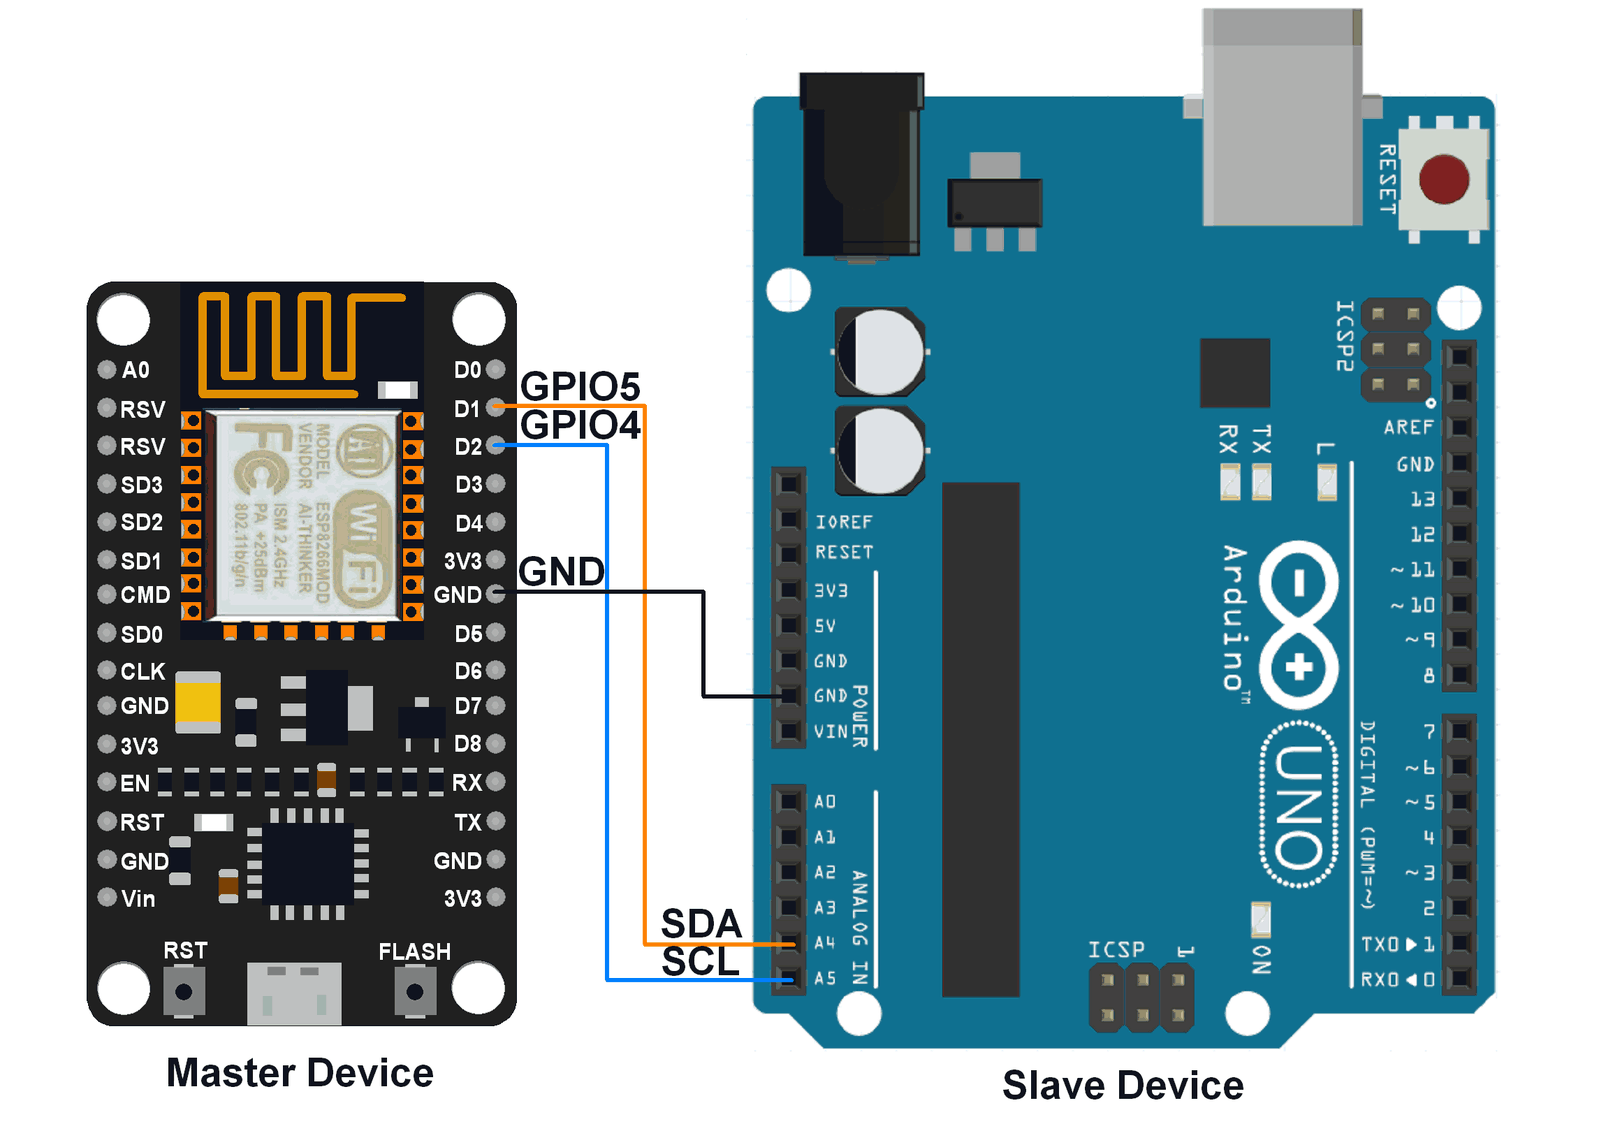
\includegraphics[angle=0, scale=.2]{Img4.png}}
\caption{Conexão da ESP8266 com o Arduino Uno.}
\label{fig4}
\end{figure}


\section{Conclusão}

Foi desenvolvida uma unidade de remota de irrigação, com o propósito de manter hortas e jardins independentemente da presença do usuário, de forma confiável e autônoma. Foram desenvolvidos programas para o microcontrolador ATmega328P capazes de fazer a contagem de tempo em escala real de forma precisa, de realizar a comunicação à distância com o usuário através da Internet e de monitorar as condições de operação do sistema e do ambiente onde este se encontra instalando, de forma a condicionar a operação e, proporcionando assim, maior eficiência. Foi realizada uma simulação bem sucedida utilizando o programa \textit{Proteus} para aferir o funcionamento do sistema principal de acionamento da válvula solenoide e construído um protótipo para teste da comunicação sem fio com a placa Arduino Uno, também bem sucedido. Os objetivos do projeto foram alcançado, embora ainda haja espaço para muito crescimento e aperfeiçoamento, podendo, com os devidos ajustes, se tornar um dispositivo viável para implementação em diversos ambientes e condições.

\begin{thebibliography}{00}
\bibitem{b1} http://mundoeducacao.bol.uol.com.br/geografia/agricultura-familiar.htm
\bibitem{b2} Galluzzi, Gea, Pablo Eyzaguirre, and Valeria Negri. "Home gardens: neglected hotspots of agro-biodiversity and cultural diversity." Biodiversity and conservation 19.13 (2010): 3635-3654.

\bibitem{b3} E. Williams. Make: AVR Programming:[learning to Write Software for Hardware]. Maker Media, 2014.
\bibitem{b4} N. Kolban. "Kolban’s Book on ESP8266." Texas, USA (2015): 1-317.
\end{thebibliography}



\end{document}
